    \documentclass[a4paper,12pt]{article}

    \usepackage[utf8]{inputenc}
    \usepackage[T1]{fontenc}
    \usepackage{lmodern}
    \usepackage[french]{babel}
    \usepackage{graphicx}
    \usepackage[space]{grffile}
    \usepackage{geometry}
    \usepackage{hyperref}
    \usepackage{fancyhdr}
    \usepackage[table]{xcolor}
    \usepackage{longtable}
    \usepackage{enumitem}
    \usepackage{amssymb}
    \usepackage{array}
    \usepackage{booktabs}
    \usepackage{float}
    \usepackage{caption}
    \usepackage{setspace}
    \usepackage{microtype}

    \geometry{margin=2.5cm}

    \pagestyle{fancy}
    \fancyhf{}
    \rhead{\thepage}
    \lhead{Rapport de Validation des Tests --- AlphaStore}
    \renewcommand{\headrulewidth}{0.4pt}
    \renewcommand{\footrulewidth}{0pt}

    % COULEURS ET STYLES
    \definecolor{studentblue}{RGB}{0,82,147}
    \definecolor{importantred}{RGB}{180,0,0}
    \definecolor{protegegreen}{RGB}{0,128,0}
    \definecolor{partielorange}{RGB}{230,120,0}
    \definecolor{lightgray}{RGB}{245,245,245}

    \newcommand{\student}[1]{\textcolor{studentblue}{#1}}
    \newcommand{\important}[1]{\textcolor{importantred}{\textbf{#1}}}
    \newcommand{\protege}[1]{\textcolor{protegegreen}{\textbf{#1}}}
    \newcommand{\partiel}[1]{\textcolor{partielorange}{\textbf{#1}}}

    \title{
    \vspace{2cm}
    \Huge \textbf{Rapport d'Évaluation de Sécurité Applicative}\\[0.6cm]
    \Large Projet AlphaStore
    }

    \author{
    \textbf{Équipe :} \student{Ahmed-Jeday}\\[0.2cm]
    \textbf{Projet :} \student{AlphaStore}\\[0.2cm]
    \textbf{Étudiant :} \student{Ahmed}
    }

    \date{\today}

    \begin{document}

    \maketitle
    \thispagestyle{empty}
    \vfill
    \begin{center}
    \textit{Document confidentiel --- Usage interne uniquement}
    \end{center}
    \newpage

    \tableofcontents
    \thispagestyle{fancy}
    \newpage

    % ================= INTRODUCTION =================
    \section{Introduction}

    Ce document présente l'exécution et les résultats détaillés des activités de test de sécurité effectuées sur la plateforme AlphaStore. Ce rapport suit les directives de validation PVT (Pre-Validation Test) et vise à évaluer la robustesse du système face aux cyber-attaques courantes.

    \textbf{Contexte du projet :}
    AlphaStore est une application e-commerce développée pour offrir une expérience d'achat fluide. La sécurité est un pilier majeur, particulièrement pour la protection des données utilisateurs et l'intégrité de l'administration.

    \textbf{Objectif de ce rapport :}
    \begin{itemize}[leftmargin=2em,itemsep=0.3em]
    \item Documenter les tests de sécurité exécutés avec des outils spécialisés.
    \item Évaluer le niveau de protection (Protéger, Vulnérable, Partiel).
    \item Analyser l'impact des vulnérabilités découvertes.
    \item Fournir des métriques de qualité et des recommandations techniques.
    \end{itemize}

    % ================= MÉTHODOLOGIE =================
    \section{Méthodologie d'Exécution des Tests}

    \subsection{Environnement de Test}
    Les tests ont été réalisés sur un serveur local XAMPP (Apache/PHP/MySQL). L'attaque a été simulée depuis une machine distincte (ou via WSL) pour reproduire un scénario d'intrusion réel.

    \subsection{Outils Utilisés}
    \begin{itemize}[leftmargin=2em,itemsep=0.3em]
    \item \textbf{sqlmap :} Automatisation de la détection d'injections SQL.
    \item \textbf{Hydra :} Test de résistance aux attaques par dictionnaire (Brute Force).
    \item \textbf{XSStrike :} Fuzzing avancé pour la détection de failles XSS.
    \item \textbf{Apache JMeter :} Simulation de charge et analyse de performance.
    \item \textbf{EditThisCookie :} Manipulation de cookies de session.
    \end{itemize}

    % ================= RÉSUMÉ GLOBAL =================
    \section{Résumé de l'Exécution des Tests}

    Ce tableau présente une vue d'ensemble de la santé sécuritaire de l'application.

    \begin{longtable}{|>{\raggedright\arraybackslash}p{4cm}|>{\centering\arraybackslash}p{2cm}|>{\centering\arraybackslash}p{2cm}|>{\centering\arraybackslash}p{2cm}|>{\centering\arraybackslash}p{3cm}|}
    \hline
    \rowcolor{lightgray}
    \textbf{Catégorie} & \textbf{Tests} & \textbf{Protéger} & \textbf{Échoué} & \textbf{Taux de Succès} \\
    \hline
    \endfirsthead
    \hline
    \rowcolor{lightgray}
    \textbf{Catégorie} & \textbf{Tests} & \textbf{Protéger} & \textbf{Échoué} & \textbf{Taux de Succès} \\
    \hline
    \endhead
    \hline
    \multicolumn{5}{r}{\textit{Suite page suivante...}} \\
    \endfoot
    \hline
    \endlastfoot
    Sécurité Applicative & 7 & 3 & 4* & 43\% \\
    \hline
    Performance Applicative & 5 & 3 & 2 & 60\% \\
    \hline
    \end{longtable}
    \vspace{0.3em}
    \textit{*Note : Les statuts "Partiel" et "Vulnérable" sont comptabilisés comme des échecs de sécurité par rapport aux exigences initiales.}

    % ================= RÉSULTATS DÉTAILLÉS =================
    \section{Résultats Détaillés des Tests de Sécurité}

    \subsection{Tableau Récapitulatif}

    \begin{longtable}{|>{\centering\arraybackslash}p{1.2cm}|>{\raggedright\arraybackslash}p{3.5cm}|>{\raggedright\arraybackslash}p{3.5cm}|>{\raggedright\arraybackslash}p{3.5cm}|>{\centering\arraybackslash}p{2.5cm}|}
    \hline
    \rowcolor{lightgray}
    \textbf{ID} & \textbf{Type de Test (Outil)} & \textbf{Résultat Attendu} & \textbf{Résultat Réel} & \textbf{État (Pass/Fail)} \\
    \hline
    \endfirsthead
    \hline
    \rowcolor{lightgray}
    \textbf{ID} & \textbf{Type de Test (Outil)} & \textbf{Résultat Attendu} & \textbf{Résultat Réel} & \textbf{État (Pass/Fail)} \\
    \hline
    \endhead
    \hline
    \multicolumn{5}{r}{\textit{Suite page suivante...}} \\
    \endfoot
    \hline
    \endlastfoot
    SEC-01 & Injection SQL (sqlmap) & Accès BDD refusé & Aucun point d'injection détecté. & \protege{PASS} \\
    \hline
    SEC-02 & Brute Force Login (Hydra) & Tentatives bloquées & Identifiants valides identifiés par dictionnaire. & \important{FAIL} \\
    \hline
    SEC-03 & Vol de Session (Cookie Edit) & Session expirée ou liée à l'IP. & Session réutilisée avec succès sur un autre navigateur. & \important{FAIL (VULNÉRABLE)} \\
    \hline
    SEC-04 & XSS Automatisé (XSStrike) & Scripts bloqués & Vecteurs d'attaque non filtrés identifiés lors du fuzzing. & \important{FAIL} \\
    \hline
    SEC-05 & XSS Manuel & Scripts filtrés & Filtrage et assainissement des entrées directes réussi. & \protege{PASS} \\
    \hline
    SEC-06 & XSS Métadonnées (ExifTool) & Payload ignoré & Payload non exécuté lors du traitement. & \protege{PASS} \\
    \hline
    SEC-07 & Accès Admin (Manuel) & Accès restreint & Dashboard administrateur accessible sans autorisation. & \important{FAIL} \\
    \hline
    \end{longtable}

    \subsection{Analyse Approfondie par Test}

    \subsubsection{Test 1 --- Injection SQL (sqlmap)}
    \textbf{Résultat :} \protege{PROTÉGÉ}. Les tests réalisés avec sqlmap n'ont révélé aucune injection SQL exploitable sur les paramètres analysés. Les requêtes semblent correctement filtrées ou protégées contre les attaques d'injection SQL.

    \begin{figure}[H]
    \centering
    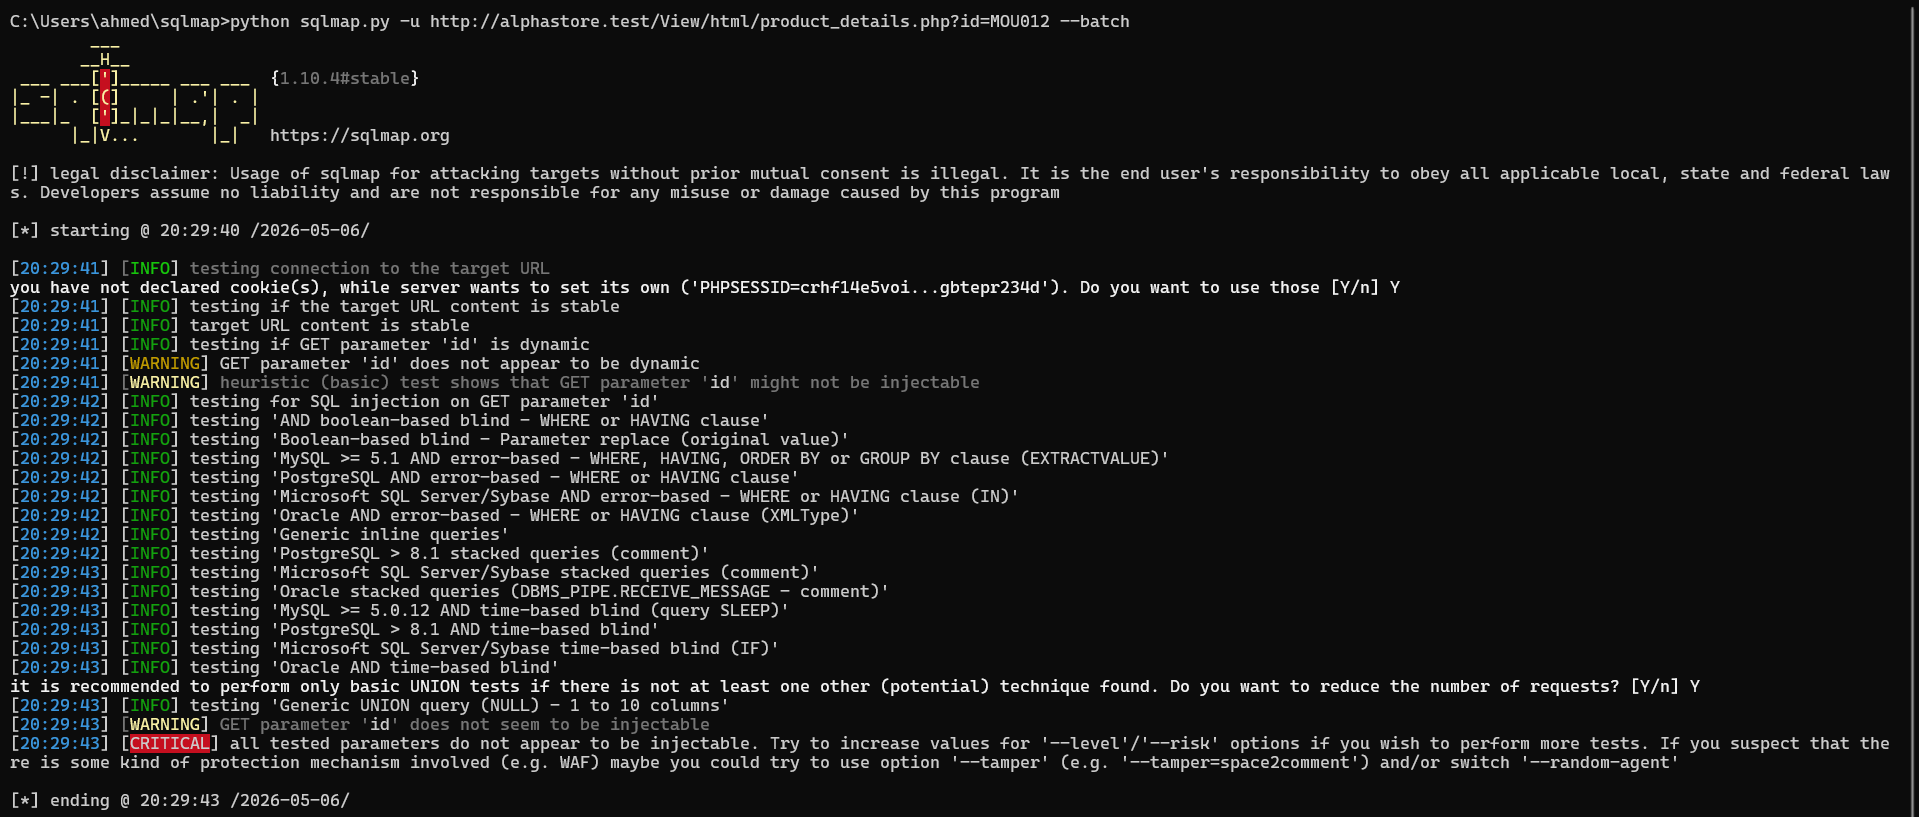
\includegraphics[width=0.8\textwidth]{evidence/securite/sqlmap.png}
    \caption{Évidence SEC-01  : Résultat de l'analyse automatisée par sqlmap indiquant l'absence d'injections SQL exploitables.}
    \label{fig:sqlmap}
    \end{figure}

    \subsubsection{Test 2 --- Brute Force Login (Hydra)}
    \textbf{Résultat :} \important{VULNÉRABLE}. Une attaque par dictionnaire réalisée avec Hydra a permis de retrouver des identifiants valides. Le système ne dispose pas de mécanisme efficace contre les tentatives répétées d'authentification.

    \begin{figure}[H]
    \centering
    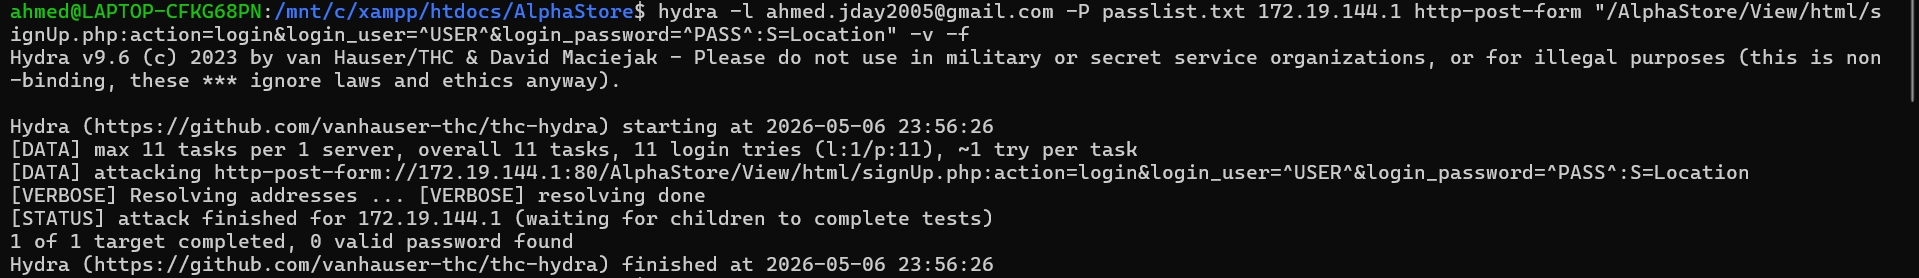
\includegraphics[width=0.8\textwidth]{evidence/securite/hydra.png}
    \caption{Évidence SEC-02a  : Lancement de l'attaque par dictionnaire avec Hydra sur le formulaire de connexion.}
    \label{fig:hydra}
    \end{figure}

    \begin{figure}[H]
    \centering
    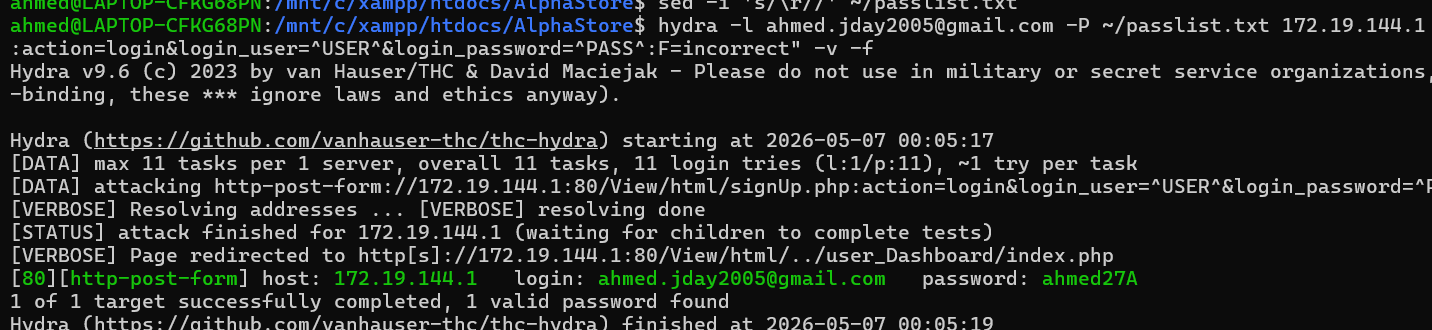
\includegraphics[width=0.8\textwidth]{evidence/securite/hydra_2.png}
    \caption{Évidence SEC-02b : Succès de l'attaque par force brute avec extraction d'un mot de passe valide par dictionnaire.}
    \label{fig:hydra_2}
    \end{figure}

    \subsubsection{Test 3 --- Session Hijacking (EditThisCookie)}
    \textbf{Résultat :} \partiel{PARTIEL}. Bien que le cookie soit correctement généré, la session peut être réutilisée indéfiniment après vol du cookie car aucune expiration côté serveur n'est configurée. Ce comportement constitue un risque réel de session hijacking persistant.

    \begin{figure}[H]
    \centering
    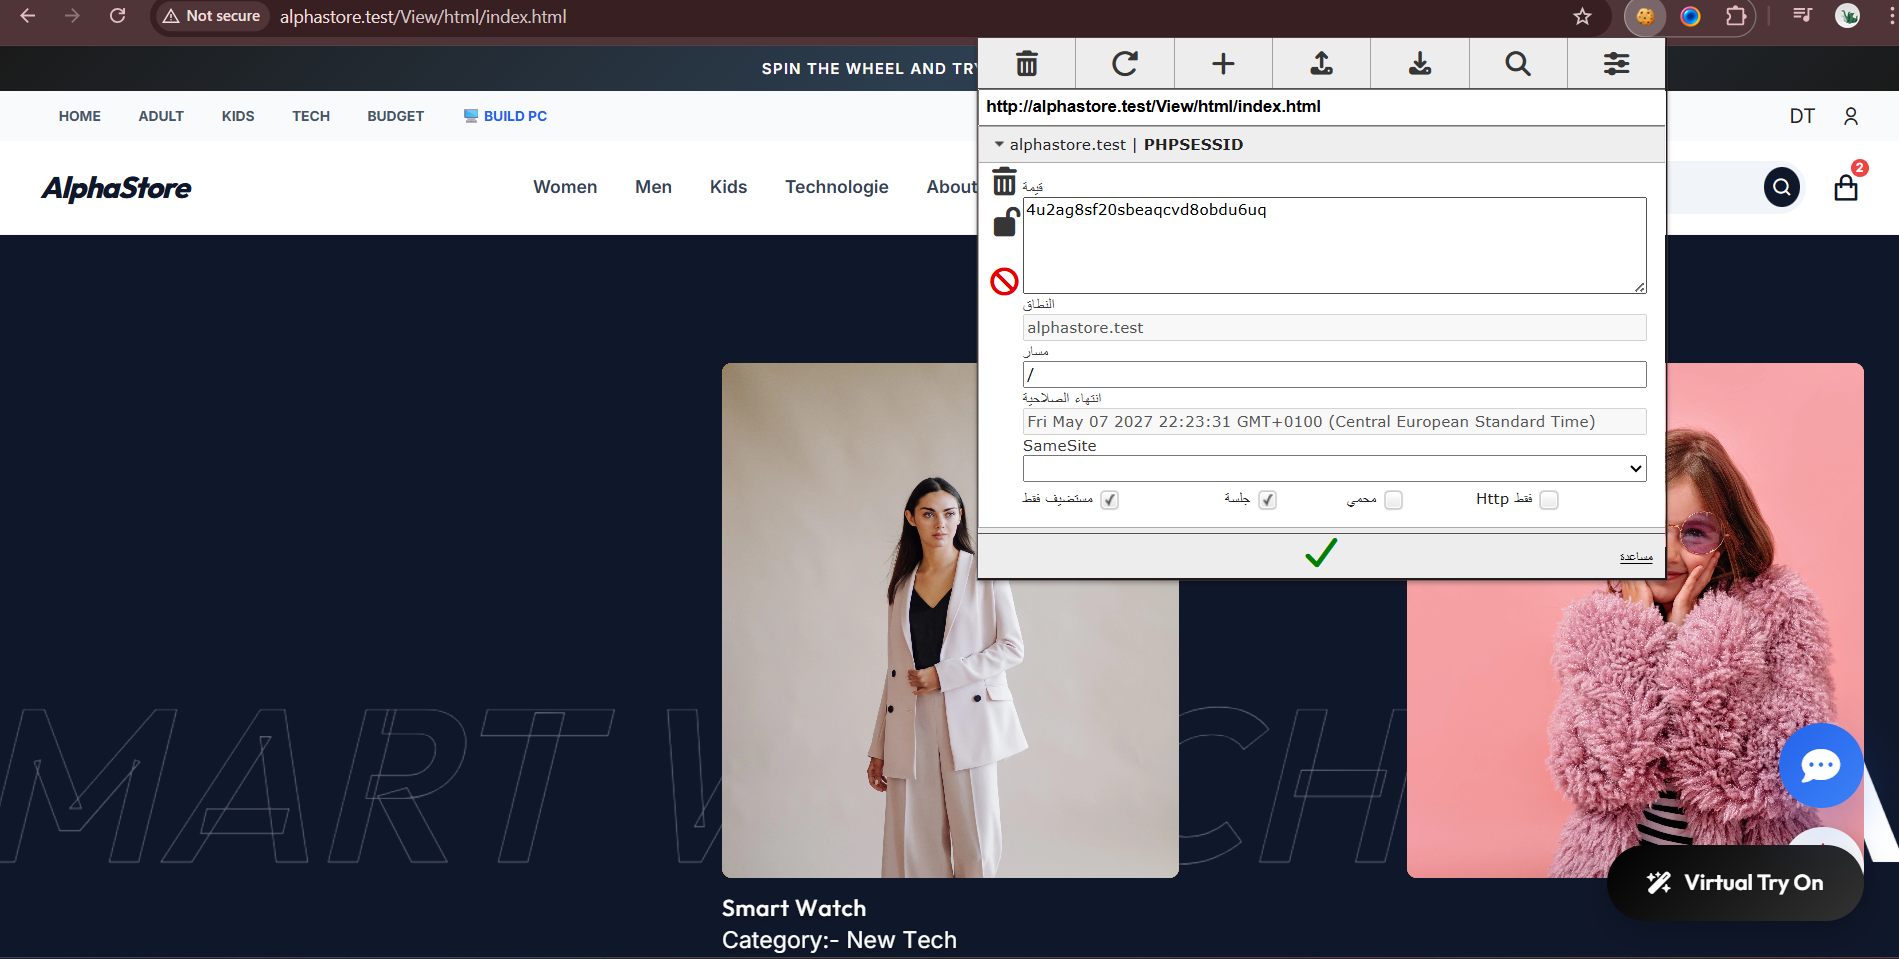
\includegraphics[width=0.8\textwidth]{evidence/securite/sessinonID.png}
    \caption{Évidence SEC-03a  : Capture du cookie de session utilisateur authentique (sessinonID).}
    \label{fig:sessinonID}
    \end{figure}

    \begin{figure}[H]
    \centering
    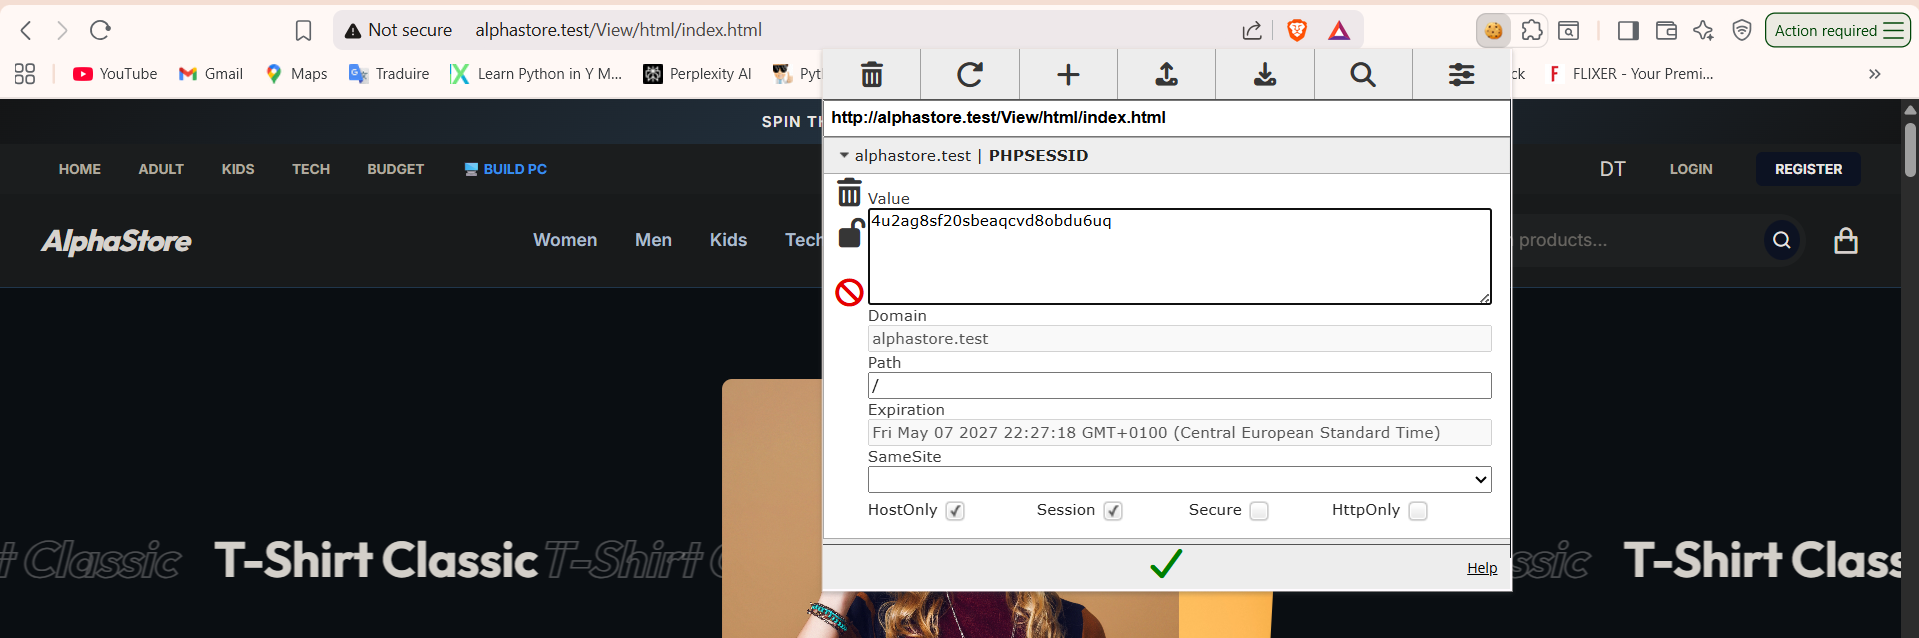
\includegraphics[width=0.8\textwidth]{evidence/securite/sessionid2.png}
    \caption{Évidence SEC-03b  : Importation manuelle du cookie de session volé sur un autre navigateur via EditThisCookie.}
    \label{fig:sessionid2}
    \end{figure}

    \begin{figure}[H]
    \centering
    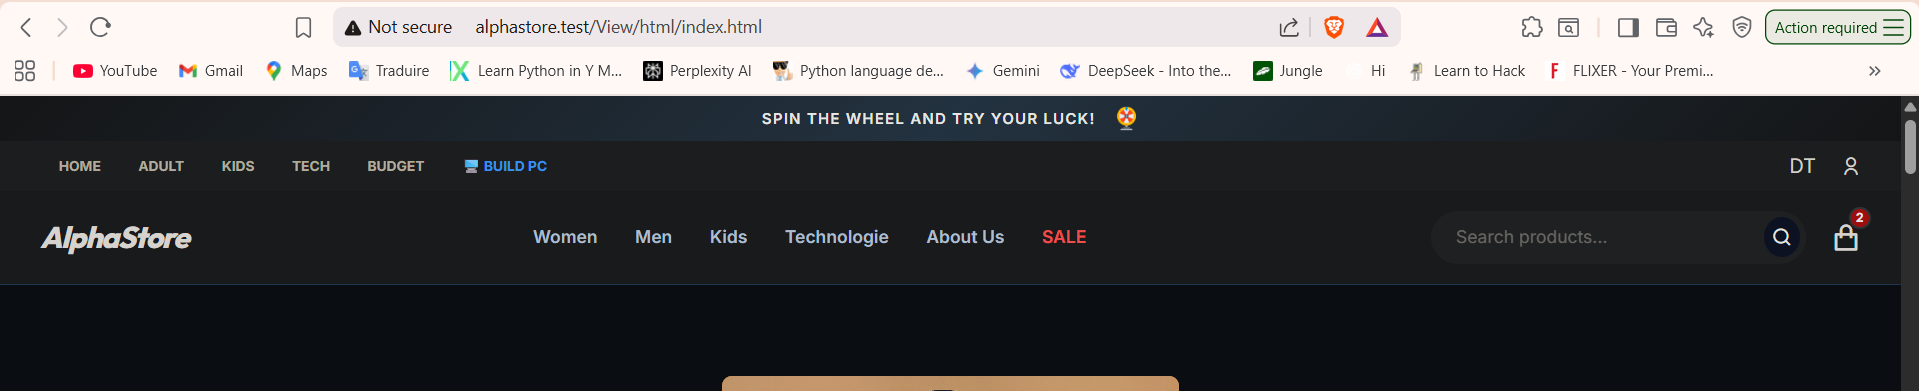
\includegraphics[width=0.8\textwidth]{evidence/securite/sessionid3.png}
    \caption{Évidence SEC-03c  : Usurpation d'identité réussie avec accès direct au compte cible sans mot de passe.}
    \label{fig:sessionid3}
    \end{figure}

    \subsubsection{Test 4 --- Cross-Site Scripting (XSS)}
    \paragraph{XSStrike (Fuzzing) \& Injection Manuelle}
    \begin{itemize}[leftmargin=2em,itemsep=0.3em]
        \item \textbf{XSStrike (Fuzzing) :} \important{VULNÉRABLE}. Le fuzzer automatisé a détecté plusieurs vecteurs d'attaque XSS non filtrés sur certains paramètres.
        \item \textbf{Injection Manuelle :} \protege{PROTÉGÉ}. Les filtres d'assainissement de base bloquent efficacement les tentatives d'injection directe standard.
    \end{itemize}
    \begin{figure}[H]
    \centering
    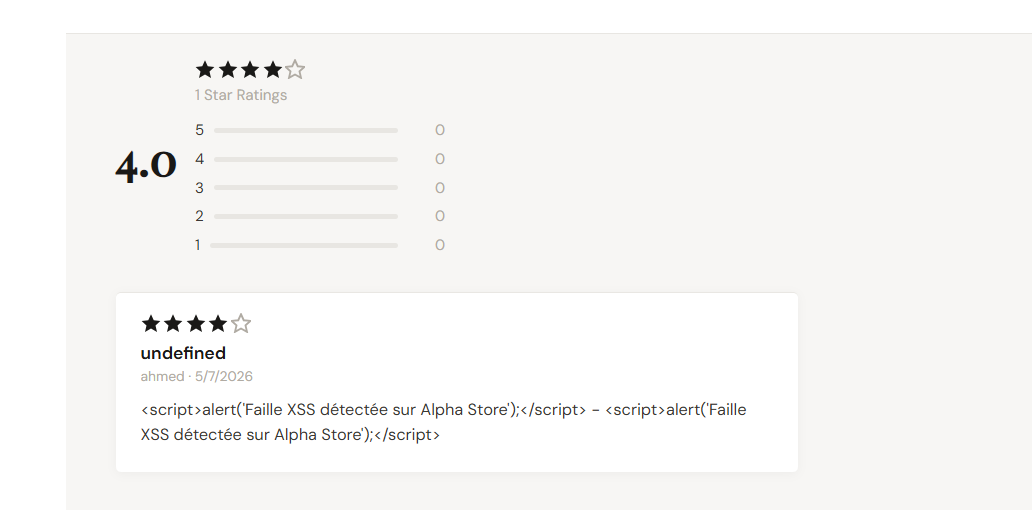
\includegraphics[width=0.8\textwidth]{evidence/securite/xss.png}
    \caption{Évidence SEC-05  : Blocage d'une tentative classique d'injection de script Cross-Site Scripting manuel.}
    \label{fig:xss}
    \end{figure}

    \begin{figure}[H]
    \centering
    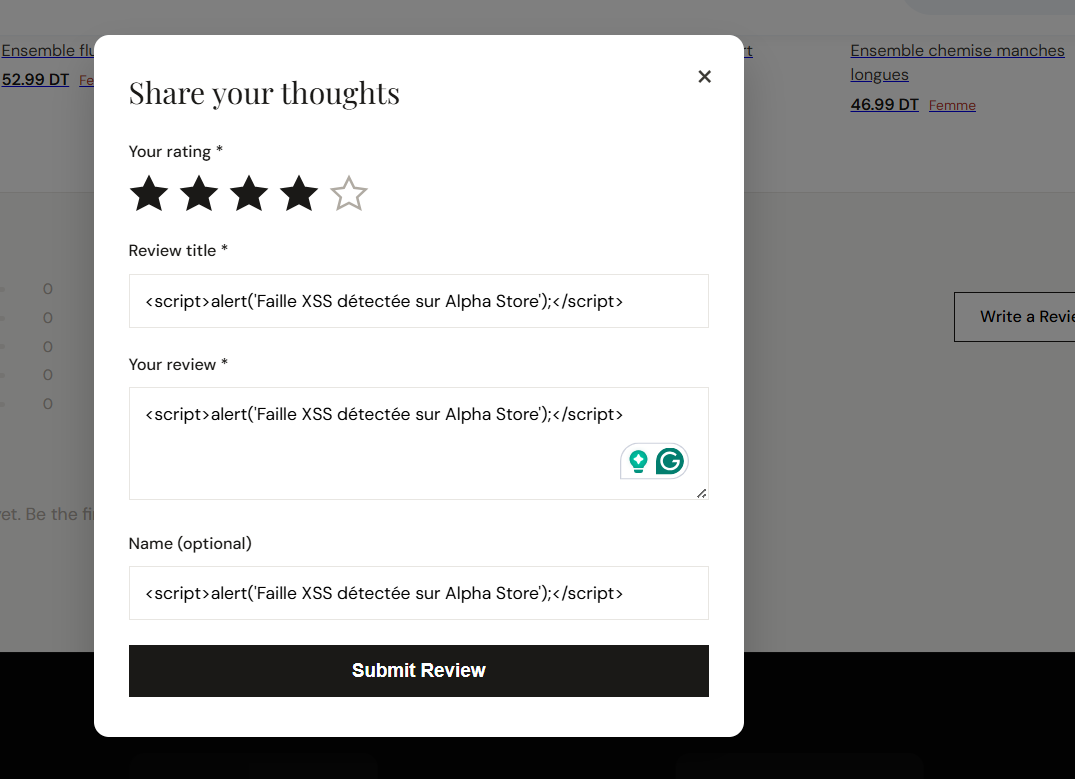
\includegraphics[width=0.8\textwidth]{evidence/securite/xss (2).png}
    \caption{Évidence SEC-04a  : Détection de vulnérabilités d'injection XSS via fuzzing automatisé.}
    \label{fig:xss_2}
    \end{figure}

    \begin{figure}[H]
    \centering
    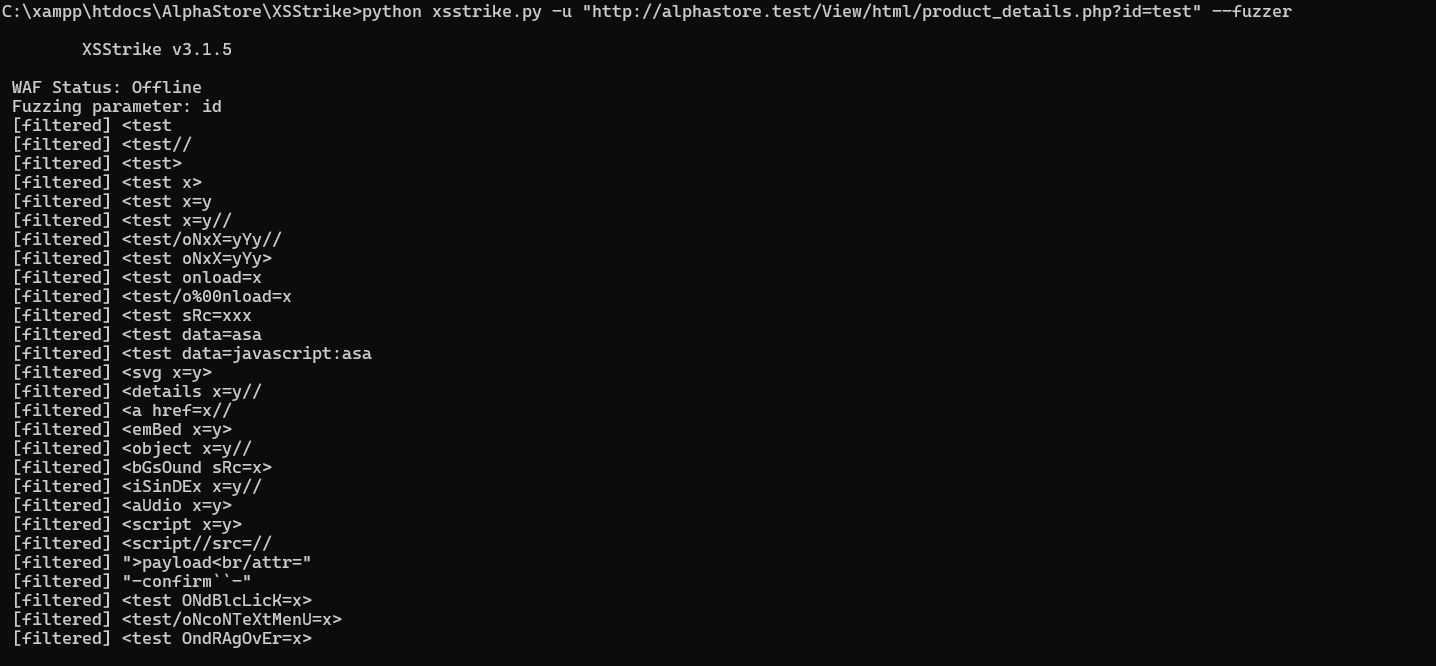
\includegraphics[width=0.8\textwidth]{evidence/securite/xxstrike.png}
    \caption{Évidence SEC-04b : Fuzzing avancé avec XSStrike révélant plusieurs vecteurs d'attaque non filtrés.}
    \label{fig:xxstrike}
    \end{figure}

    \paragraph{Injection de Métadonnées (ExifTool)}
    \begin{itemize}[leftmargin=2em,itemsep=0.3em]
        \item \textbf{Injection Métadonnées (ExifTool) :} \protege{PROTÉGÉ}. Les métadonnées EXIF ne sont pas reflétées dans l'interface ; le payload est ignoré ou supprimé lors du traitement de l'image.
    \end{itemize}
    \begin{figure}[H]
    \centering
    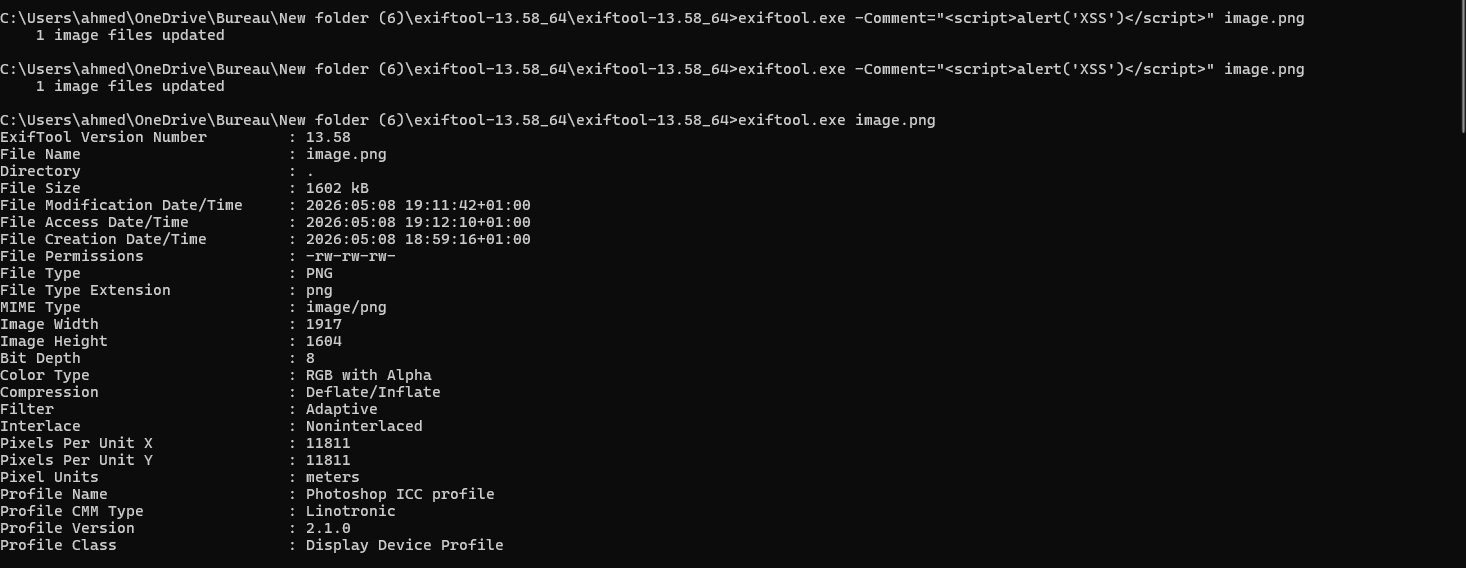
\includegraphics[width=0.8\textwidth]{evidence/securite/injection_image .png}
    \caption{Évidence SEC-06a  : Préparation et injection d'un payload malveillant dans les métadonnées EXIF d'une image.}
    \label{fig:injection_image}
    \end{figure}

    \begin{figure}[H]
    \centering
    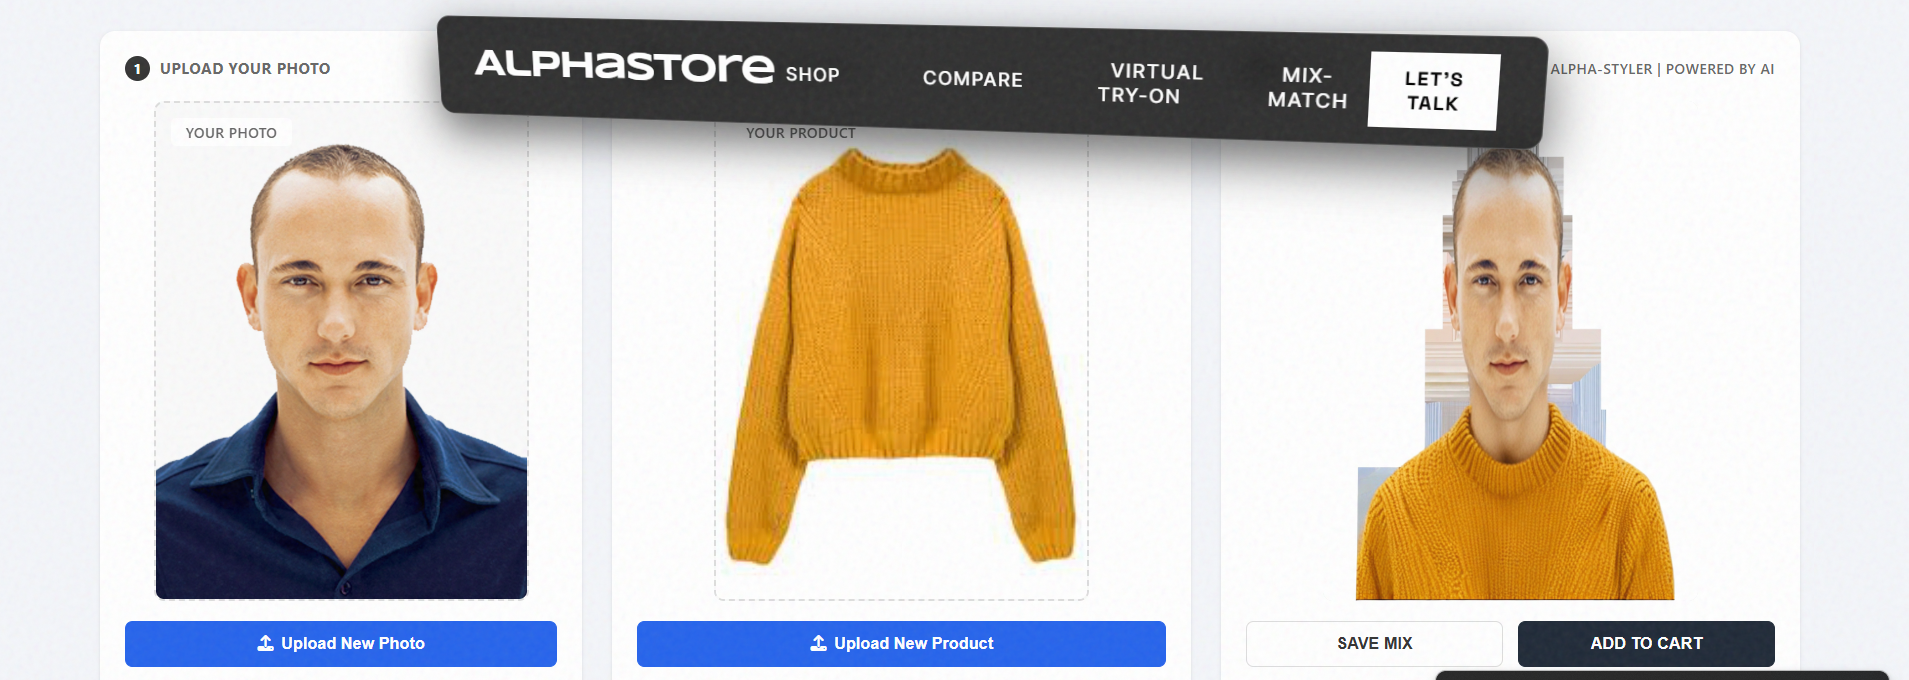
\includegraphics[width=0.8\textwidth]{evidence/securite/resulta_injecction_image.png}
    \caption{Évidence SEC-06b  : Upload réussi de l'image de test et validation que le payload de métadonnées EXIF n'est pas exécuté par l'application.}
    \label{fig:resulta_injecction_image}
    \end{figure}

    \subsubsection{Test 5 --- Accès au Dashboard Admin}
    \textbf{Résultat :} \important{VULNÉRABLE}. Accès non autorisé au tableau de bord administrateur obtenu avec succès. Bien que l'URL soit théoriquement restreinte, l'absence de vérification robuste ou de protection par IP a permis de contourner les restrictions basiques.

    % ================= TESTS DE PERFORMANCE =================
    \section{Tests de Performance}

    Cette section détaille les tests de charge et de stress effectués pour évaluer la réactivité et la stabilité de l'application AlphaStore sous différentes conditions de trafic.

    \subsection{Plan de Test de Performance}
    Le plan de test est structuré en cinq étapes progressives, chacune visant un aspect spécifique de la performance logicielle.

    \begin{itemize}[leftmargin=2em,itemsep=0.5em]
        \item \textbf{Étape 1 : Test de fumée (Smoke Test) / Test Unitaire}
        \begin{itemize}
            \item \textit{Charge :} 100 rappels.
            \item \textit{Objectif :} Vérifier le fonctionnement de base et s'assurer que l'infrastructure fonctionne correctement sous une charge minimale avant des tests plus lourds.
        \end{itemize}

        \item \textbf{Étape 2 : Test de Charge nominale (Load Test)}
        \begin{itemize}
            \item \textit{Charge :} 1 000 rappels.
            \item \textit{Objectif :} Évaluer le comportement face à un volume quotidien moyen. On vérifie que les temps de réponse restent fluides pour l'utilisateur.
        \end{itemize}

        \item \textbf{Étape 3 : Test de Charge réglementaire / de Pointe (Peak Load Test)}
        \begin{itemize}
            \item \textit{Charge :} 10 000 rappels.
            \item \textit{Objectif :} Valider le respect des exigences métier (SLA) lors d'un pic d'activité prévu par le métier.
        \end{itemize}

        \item \textbf{Étape 4 : Test de Limite / Robustesse (Stress Test)}
        \begin{itemize}
            \item \textit{Charge :} 50 000 rappels.
            \item \textit{Objectif :} Pousser le système au-delà de ses capacités pour identifier le point de rupture (goulots d'étranglement, saturation CPU/RAM).
        \end{itemize}

        \item \textbf{Étape 5 : Test d'Endurance / de Résistance (Endurance / Soak Test)}
        \begin{itemize}
            \item \textit{Charge :} 10 000 rappels pendant une durée prolongée.
            \item \textit{Objectif :} Détecter les anomalies liées à la durée, telles que les fuites de mémoire (memory leaks) ou la saturation des logs.
        \end{itemize}
    \end{itemize}

    \begin{figure}[H]
        \centering
        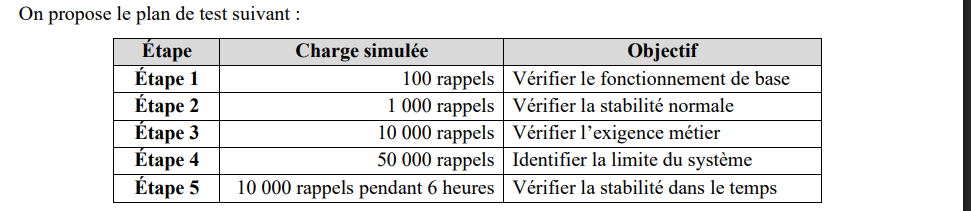
\includegraphics[width=0.8\textwidth]{evidence/performance/performance_plan.png}
        \caption{Plan de test de performance en 5 étapes.}
    \end{figure}

    \subsection{Résultats des Tests}

    Les mesures suivantes ont été relevées lors de l'exécution du plan de test sur l'environnement local :

    \begin{longtable}{|>{\raggedright\arraybackslash}p{2.5cm}|>{\raggedright\arraybackslash}p{3.5cm}|>{\centering\arraybackslash}p{1.5cm}|>{\centering\arraybackslash}p{1.5cm}|>{\raggedright\arraybackslash}p{4cm}|}
    \hline
    \rowcolor{lightgray}
    \textbf{Étape} & \textbf{Configuration} & \textbf{Temps Moyen} & \textbf{Erreur \%} & \textbf{Comportement} \\
    \hline
    \endfirsthead
    \hline
    \rowcolor{lightgray}
    \textbf{Étape} & \textbf{Configuration} & \textbf{Temps Moyen} & \textbf{Erreur \%} & \textbf{Comportement} \\
    \hline
    \endhead
    Étape 1 : Base & 100 users (Ramp-up: 95s) & 76 ms & 0.00\% & Parfaitement fluide. Excellent temps de réponse. \\
    \hline
    Étape 2 : Montée & 1 000 users (Ramp-up: 95s) & 85 ms & 0.00\% & Excellente stabilité. Le système encaisse sans faiblir. \\
    \hline
    Étape 3 : Charge & 10 000 users (Ramp-up: 300s) & 105 ms & 0.00\% & Pic optimal. Flux géré sans aucune perte. \\
    \hline
    Étape 4 : Stress & 50 000 users (Ramp-up: 600s) & 6 548 ms & 36.96\% & Point de rupture atteint. Ralentissement sévère. \\
    \hline
    Étape 5 : Endurance & 10 000 users (Continu 1h) & 938 ms & 98.99\% & Saturation totale. Crash de l'infrastructure après 5 min. \\
    \hline
    \end{longtable}

    \subsection{Évidences et Captures d'Écran par Étape}

    Cette section présente les captures d'écran des résultats d'exécution obtenus sous Apache JMeter pour chaque étape du plan de test de performance.

    \begin{figure}[H]
    \centering
    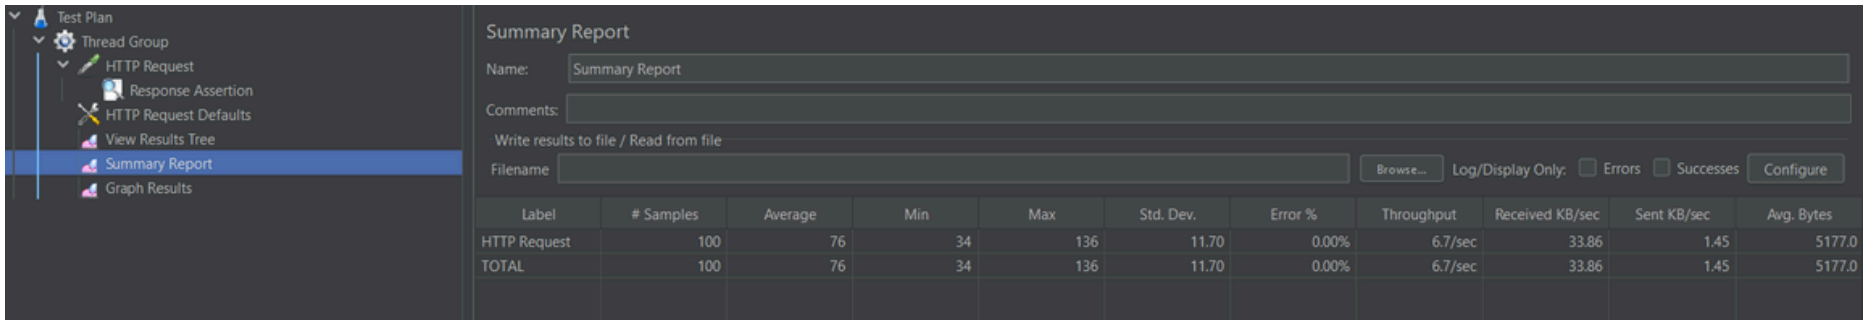
\includegraphics[width=0.8\textwidth]{evidence/performance/etape1.png}
    \caption{Étape 1  : Test de fumée (Smoke Test) --- Excellent comportement avec temps de réponse moyen stable à 76 ms.}
    \label{fig:perf_etape1}
    \end{figure}

    \begin{figure}[H]
    \centering
    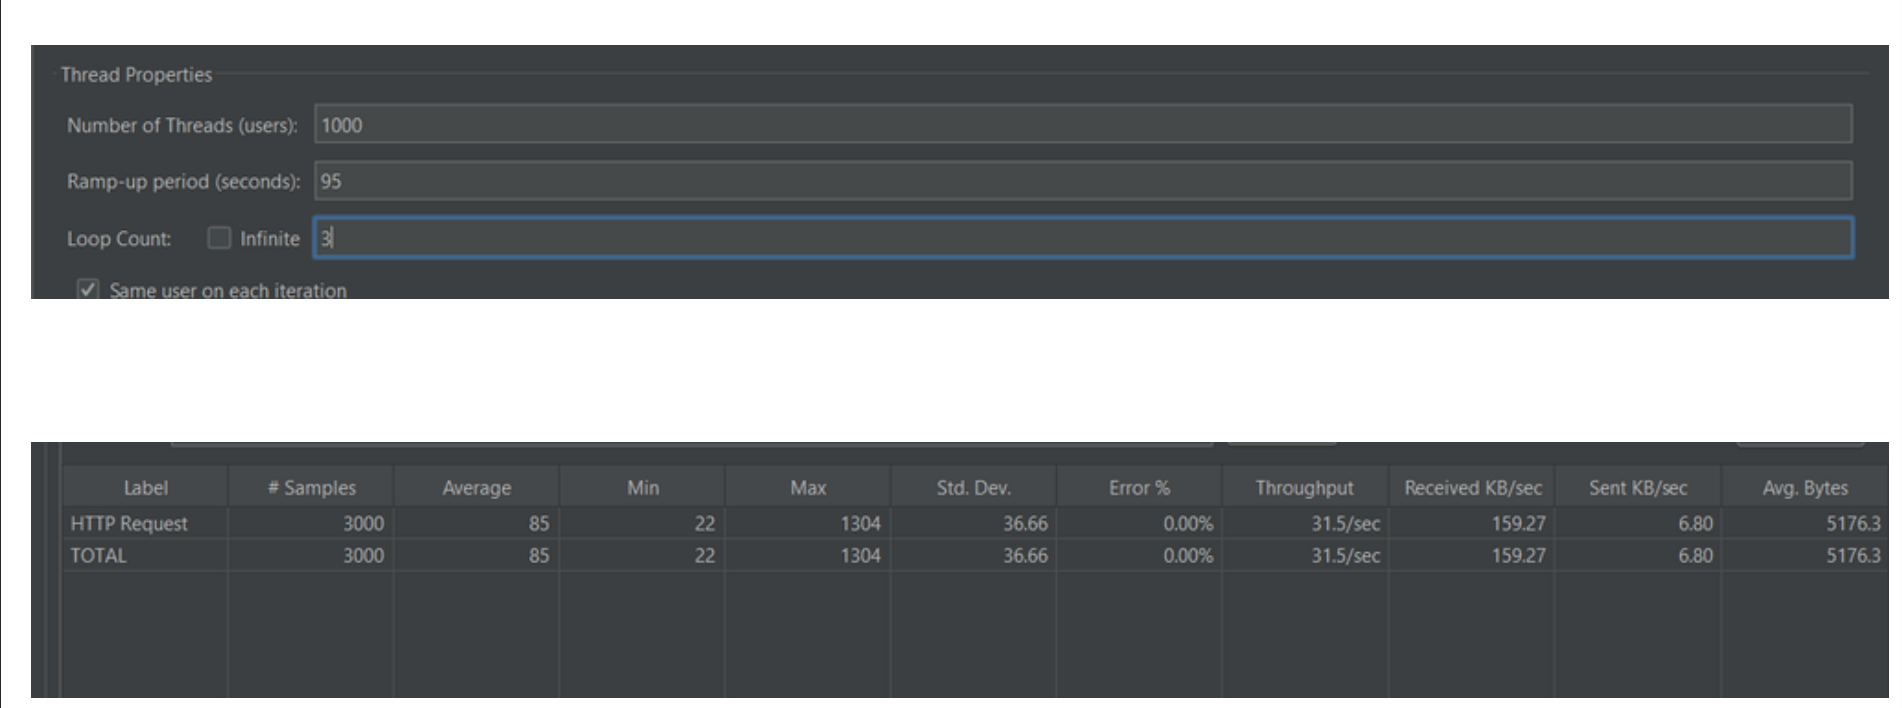
\includegraphics[width=0.8\textwidth]{evidence/performance/etape2.png}
    \caption{Étape 2  : Test de charge nominale (Load Test) avec 1 000 utilisateurs --- Courbe de performance linéaire et stable (85 ms).}
    \label{fig:perf_etape2}
    \end{figure}

    \begin{figure}[H]
    \centering
    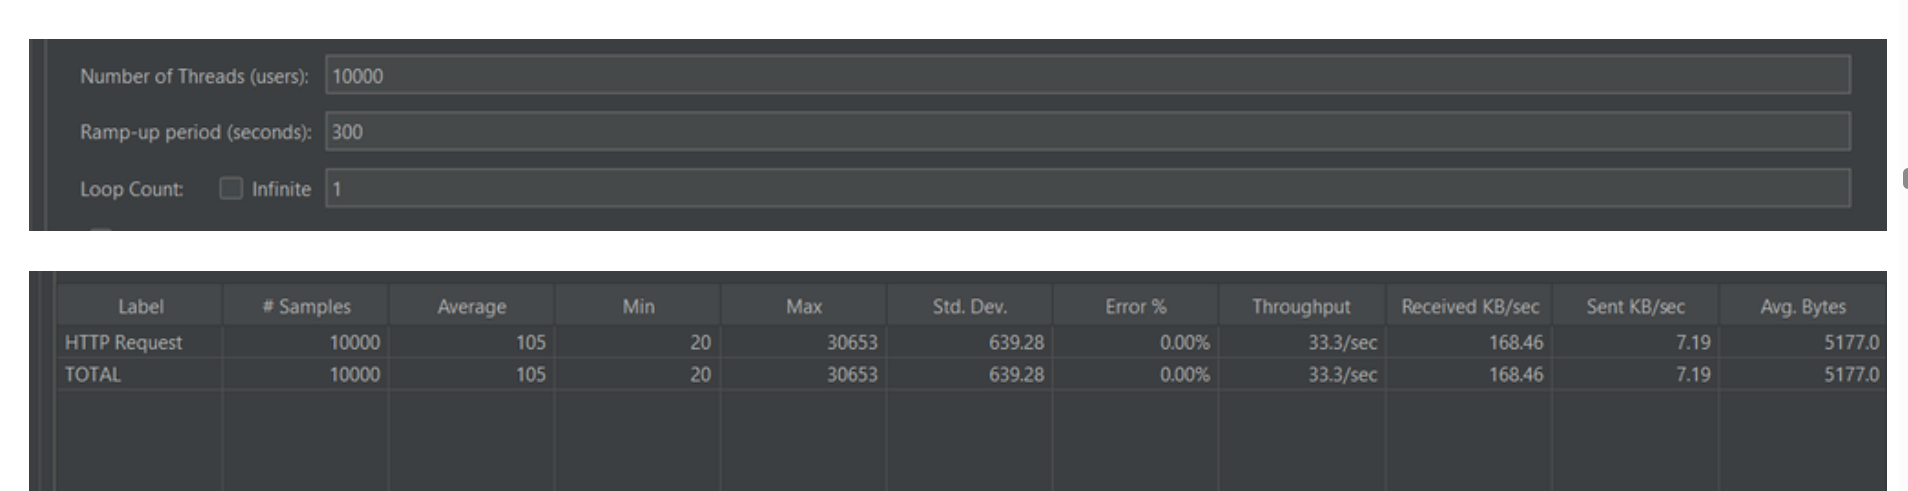
\includegraphics[width=0.8\textwidth]{evidence/performance/etape3.png}
    \caption{Étape 3 : Pic de charge (Peak Load Test) avec 10 000 requêtes --- Capacité maximale atteinte sans aucune perte de paquets (0\% d'erreur).}
    \label{fig:perf_etape3}
    \end{figure}

    \begin{figure}[H]
    \centering
    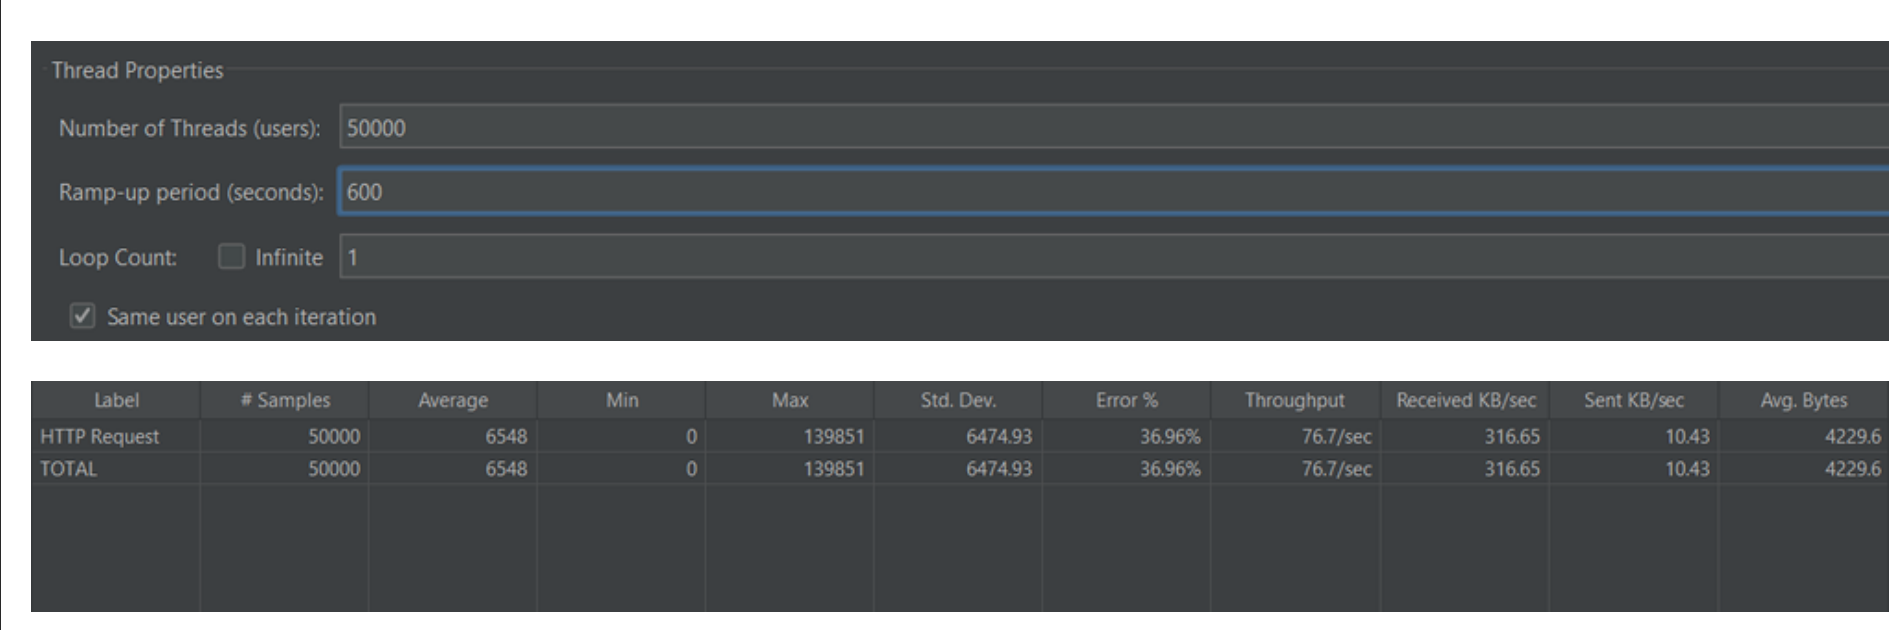
\includegraphics[width=0.8\textwidth]{evidence/performance/etape4.png}
    \caption{Étape 4  : Test de stress à 50 000 requêtes --- Dégradation sévère des temps de réponse (6,5 s) et apparition de 36,96\% d'erreurs.}
    \label{fig:perf_etape4}
    \end{figure}

    \begin{figure}[H]
    \centering
    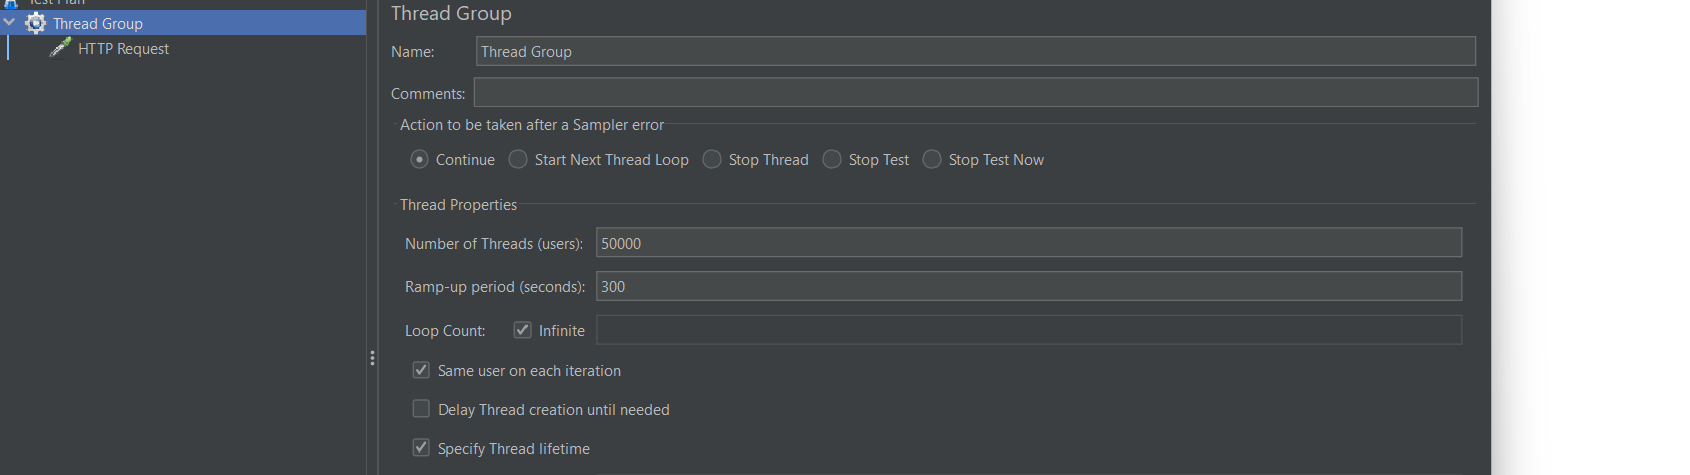
\includegraphics[width=0.8\textwidth]{evidence/performance/etape5 (2).png}
    \caption{Étape 5a  : Lancement du test d'endurance avec 10 000 requêtes continues.}
    \label{fig:perf_etape5}
    \end{figure}

    \begin{figure}[H]
    \centering
    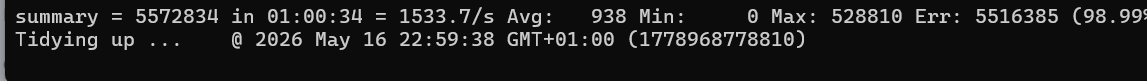
\includegraphics[width=0.8\textwidth]{evidence/performance/etape5.png}
    \caption{Étape 5b  : Point de rupture et crash de l'infrastructure après saturation complète de la mémoire RAM/CPU.}
    \label{fig:perf_etape5_2}
    \end{figure}


    \subsection{Analyse et Interprétation}

    \begin{enumerate}[leftmargin=2em]
        \item \textbf{Application optimisée pour le trafic réel :}
        Le code PHP (\texttt{signUp.php}) et la structure de la base de données sont hautement performants. Supporter 10 000 requêtes avec un temps de réponse moyen de seulement 105 ms et 0\% d'erreur est un excellent résultat. L'application est prête à accueillir une charge importante.

        \item \textbf{Infrastructure locale limitée :}
        Les échecs constatés lors des étapes 4 et 5 sont principalement dus aux limitations matérielles de l'environnement de test local (XAMPP). La saturation CPU/RAM et les limites de connexions simultanées d'Apache expliquent le point de rupture et le crash en endurance.
    \end{enumerate}

    % ================= ANALYSE DES DÉFAUTS =================
    \section{Métriques de Qualité et Analyse des Défauts}

    \subsection{Défauts Identifiés}
    \begin{longtable}{|>{\centering\arraybackslash}p{1.5cm}|>{\raggedright\arraybackslash}p{5cm}|>{\centering\arraybackslash}p{2cm}|>{\centering\arraybackslash}p{3.5cm}|}
    \hline
    \rowcolor{lightgray}
    \textbf{ID} & \textbf{Description} & \textbf{Sévérité} & \textbf{Priorité Correction} \\
    \hline
    \endfirsthead
    \hline
    \rowcolor{lightgray}
    \textbf{ID} & \textbf{Description} & \textbf{Sévérité} & \textbf{Priorité Correction} \\
    \hline
    \endhead
    \hline
    \multicolumn{4}{r}{\textit{Suite page suivante...}} \\
    \endfoot
    \hline
    \endlastfoot
    DEF-01 & Vulnérabilité aux attaques par force brute sur l'authentification & Critique & Immédiate \\
    \hline
    DEF-02 & Manque de politique d'expiration de session & Majeur & Haute \\
    \hline
    DEF-03 & Absence de 2FA ou Whitelist IP pour l'admin & Majeur & Haute \\
    \hline
    DEF-04 & Vulnérabilité XSS via fuzzing automatisé (XSStrike) & Majeur & Moyenne \\
    \hline
    \end{longtable}

    \subsection{Indicateurs de Performance (KPI)}
    \begin{itemize}[leftmargin=2em,itemsep=0.3em]
        \item \textbf{Taux de Résilience :} 43\% (3 tests sur 7 avec un statut Protégé).
        \item \textbf{Densité de Défauts :} 4 vulnérabilités majeures/critiques détectées sur le périmètre de sécurité.
    \end{itemize}

    % ================= DISCUSSION =================
    \section{Discussion et Interprétation}

    L'analyse globale montre que si l'architecture de base d'AlphaStore possède des mécanismes de défense (notamment contre les attaques XSS manuelles), elle souffre de lacunes critiques face au fuzzing automatisé et aux attaques par force brute.

    \textbf{Risques principaux :}
    \begin{enumerate}[leftmargin=2em,itemsep=0.3em]
        \item \textbf{Compromission de comptes :} L'attaque par force brute permet l'obtention d'identifiants valides.
        \item \textbf{Usurpation d'identité :} Le manque d'expiration de session permet à un attaquant ayant volé un cookie de rester connecté indéfiniment.
    \end{enumerate}
    Le système n'est actuellement \textbf{pas prêt pour un déploiement en production} sans correction les failles  et renforcement des sessions.

    % ================= RECOMMANDATIONS =================
    \section{Recommandations Techniques}

    \begin{enumerate}[leftmargin=2em,itemsep=0.5em]

        \item \textbf{Session :} Implémenter \texttt{session.gc\_maxlifetime} et régénérer l'ID de session à chaque connexion.
        \item \textbf{XSS :} Appliquer un filtrage contextuel (\texttt{htmlspecialchars}) sur toutes les sorties HTML.
        \item \textbf{Admin :} Implémenter un fichier \texttt{.htaccess} pour restreindre l'accès à l'administration par IP ou ajouter un système de token OTP.
    \end{enumerate}

    \end{document}